\documentclass[xcolor=svgnames]{beamer}

\usepackage{algorithmic}
\usepackage[ruled]{algorithm2e}
\usepackage[utf8]    {inputenc}
\usepackage[T1]      {fontenc}
\usepackage[english] {babel}
\usepackage{todonotes}
\usepackage{amsmath,amsfonts,graphicx}
\usepackage{beamerleanprogress}
\usepackage{hyperref}
\usepackage{listings}	
\usepackage{adjustbox}
\usepackage{ragged2e}

\usefonttheme[onlymath]{serif}

\newcommand{\introframe}[2]{
    \begin{frame}
	   \vfill
	   \hfill\Huge{#1}
	   
	   \vspace{1em}
	   
	   \hfill\Large{#2}
	   \vfill
    \end{frame}
}

\addtobeamertemplate{navigation symbols}{}{%
    \usebeamerfont{footline}%
    \usebeamercolor[fg]{footline}%
    \hspace{1em}%
%    \insertframenumber/\inserttotalframenumber
}


\title{Artificial Immune Systems}

\author[Aires, Amado, Chang, Collioni, Macedo]
    {
        João Paulo Aires\and
        Leonardo Amado\and
        Stephan Chang\\ \vspace{0.25em}
        Alessandro Collioni\and
        Rafael Macedo
    }

\date{November 12, 2015}

\institute
    {
        Pontifical Catholic University of Rio Grande do Sul, PUCRS\\
        Porto Alegre -- Brazil
    }

\begin{document}

    \maketitle

	\introframe{Introduction}{What is it and why use it?}
	
	\begin{frame}{Artificial Immune Systems}
        \textbf{What are they?}
        
        \begin{itemize}
            \item AIS is the product of Immune Engineering;
				\item Immune Engineering develops models that are inspired by the Immune System;
            \item Multiple models of the Immune System serve as  metaphors to solve different kinds of problems.
        \end{itemize}        
    \end{frame}
    
    \begin{frame}{Artificial Immune Systems}            
        \textbf{What are they not?}
        
        \begin{itemize}
            \item AIS is not supposed to be a computational reconstruction of the immune system;
            \item Evolutionary Algorithms (although they can be used within AIS)
        \end{itemize}    
	\end{frame}
    	
        \begin{frame}{Artificial Immune Systems}
            \only<1>{\textbf{How can we apply AIS?}}
            \only<2>{\textbf{It even reaches outside Computer Science.}}
        	\begin{itemize}
                \only<1>{\item We use the Immune System as a metaphor to solve problems;
                \item There are many theories behind the Immune System;
                \item Depending on the theory, different applications may ensue, \textit{e.g.} Information Security, Anomaly Detection, Pattern Recognition, Data Mining, Machine Learning.}
			    \only<2>{
                    \item We use the immune system as a metaphor to solve problems.
    			    \item Computer Engineers try to reproduce the immune system for computer security.
    				\item Immunologists use computational models and mathematics to understand how the immune system works.}
         	\end{itemize}
    	\end{frame}
	
	\introframe{Immunology Basics}{Straight from the Natural World}
	
        \begin{frame}{The Natural Immune System}        
            \begin{itemize}
                \item Innate Immune System
                \begin{itemize}
                    \item Most basic immune response;
                    \item Present in all living beings.
                \end{itemize}
                \item Adaptive Immune System
                \begin{itemize}
                    \item Immunological memory;
                    \item Learns new patterns of attacks and pathogens;
                    \item Present in vertebrates only.
                \end{itemize}
            \end{itemize}
	    \end{frame}
        
        \begin{frame}{Immunology Basics}
            A few important types of cells to keep in mind:
            \vspace{1em}
            % SC: I see no reason why we should take 9 slides just to show this hierarchy
            % SC: In fact, I see not reason why we should introduce this hierarchy at all. AIS abstracts all of these.
        	\begin{itemize}
        	    \item Leukocytes (from the Innate IS)
                \item B-Cells (makes Memory cells)
            	\item T-Cells (activate immune responses)
         	\end{itemize}
    	\end{frame}

%    	\begin{frame}{Immunology Basics}
%            \textbf{B-Cells}
%            \vspace{1em}
%            \begin{itemize}
%                \item Originated and matured in the Bone Marrow;
%                \item Contains receptors which identify pathogens;
%                \item Offers three types of response:
%                    \begin{itemize}
%                        \item Fast-Weak (plasmablast)
%                        \item Longterm-Strong (plasma)
%                        \item Fastest-Strongest (memory)
%                    \end{itemize}
%            \end{itemize}
%        \end{frame}
%        
%        \begin{frame}{Immunology Basics}
%          \textbf{T-Cells}
%          \vspace{1em}
%          \begin{itemize}
%              \only<1>{\item Originated in the bone marrow
%              % SC: All cells are originated in the bone marrow, the difference is that B-cells are already matured by the time they exit the bone marrow, whereas T-Cells are sent to the Thymus for maturation via negative selection.
%              \item Matured in the Thymus
%          	  \item Captures signals from B-Cells' receptors
%          	  \item Helps B-Cells differentiate}
%              \only<2>{\item Reacts to viruses and tumour cells
%          	  \item Suppress other auto-reactive immune cells
%          	  \item Takes care of lingering infection elements}
%          \end{itemize}
%        \end{frame}
                         
        \begin{frame}{Immunology Basics}
            \textbf{How does an immune response work?}
            
            \begin{itemize}
                \item Pathogen enters the environment;
                \pause
                \item B-Cell receptors recognise pathogens;
                \pause
                \item Immune cells are called to arms;
                \pause
                \item Pathogen is destroyed;
                \pause
                \item Lingering infected cells are destroyed;
                \pause
                \item Strong responses are memorised.
            \end{itemize}
        \end{frame}
        
        \begin{frame}{Immunology Basics}
            \textbf{It all comes down to:}
        
            \begin{itemize}
                \item Host system defence
                \item Pattern recognition
                \item Information collection (memory cells!)
            \end{itemize}
        \end{frame}
        
        \begin{frame}{Immunology Basics}
            \only<1>{\textbf{But how do they recognise each other? Is it love?}}
            \only<2->{\textbf{NO!} There is no love. It is purely chemistry.}
            \vspace{1em}
            \pause
            \begin{itemize}
                \item Each receptor/pathogen has a shape;
                \item When these shapes are complementary, they match!
                \item The more complementary the shapes are, the higher the affinity between recogniser and recognised;
                \item The terms ``epitope'' and ``paratope'' are used to refer to the recognised and recogniser, respectively.
            \end{itemize}
        \end{frame}
        
        \begin{frame}{Immunology Basics}
            \begin{figure}
                \centering
                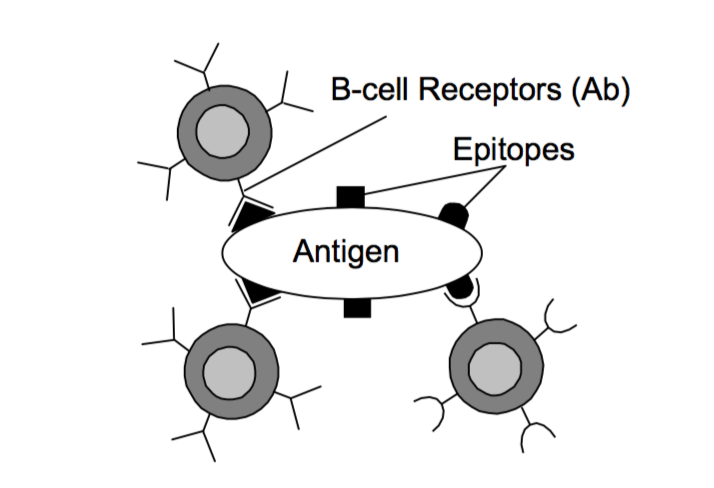
\includegraphics[width=0.75\textwidth]{fig/recognition}
                \caption{Recognition process between receptors (antibodies) and pathogens (antigens).}
            \end{figure}
        \end{frame}
        
        \begin{frame}{Immunology Basics}
            \begin{figure}
                \centering
                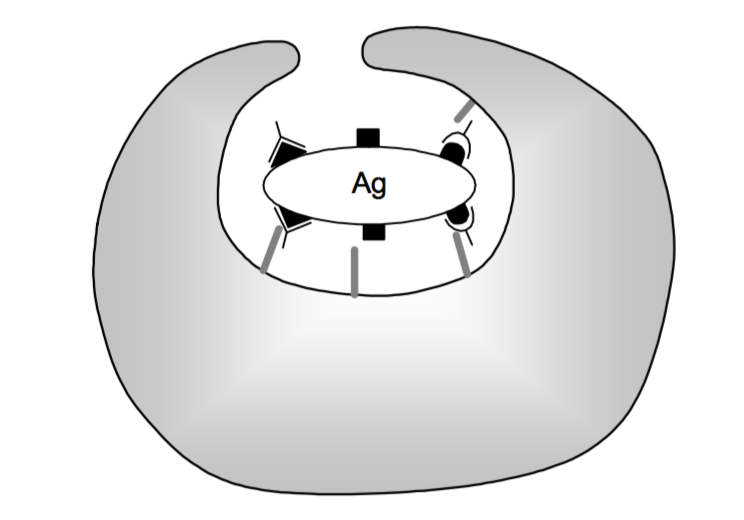
\includegraphics[width=0.7\textwidth]{fig/phagocytosis}
                \caption{When the antigen is overwhelmed, the cavalry arrives to save the day. The depicted cell is a phagocyte.}
            \end{figure}
        \end{frame}
        

    
    
    \introframe{Artificial Immune Systems}{Representation and General Principles}
    
        \begin{frame}{The Three Principles}

            \textbf{To model an AIS, we need to formalise the following elements:}

            \begin{itemize}
                \item Encoding
                \item Similarity
                \item Adaptation
                \begin{itemize}
                    \item Selection
                    \item Mutation
                \end{itemize}
            \end{itemize}
        \end{frame}

		\begin{frame}{Encoding}
            
            \textbf{Encoding is the task of translating shape-spaces to computation form.}
            
            \vspace{1em}
            The most general way to do so is with \textbf{data structures}:
            
            \vspace{0.5em}
        	
			\begin{center}
				$\begin{array}{ll}
					Ag = \langle Ag_1,Ag_2,Ag_3,...,Ag_L \rangle \cr
					Ab = \langle Ab_1,Ab_2,Ab_3,...,Ab_L \rangle \cr
                 \end{array}$
            \end{center}            
		\end{frame}
        
        \begin{frame}{Encoding}
            
            \vspace{0.5em}
            
            A shape-space can be of different types, such as:
            
            \vspace{0.5em}
            
            \begin{itemize}
            	\item Binary;
                \begin{itemize}
					\item $Ag = \langle 0,1,0,0,1,0,1 \rangle$
				\end{itemize}
                \vspace{0.3em}
				\item Integer;
               	\begin{itemize}
					\item $Ag = \langle 0, 20, 4, 5, 5, 12 \rangle$
				\end{itemize}
                \vspace{0.3em}                
                \item Real valued;
                \begin{itemize}
					\item $Ag = \langle 8.2, 7.7, 2.2, 4.8 \rangle$
				\end{itemize}
                \item Symbolic
                \begin{itemize}
					\item $Ag = \langle \langle age, 20 \rangle, \langle height, 1.7\rangle , \langle eyes,``Brown''\rangle \rangle$
				\end{itemize}
			\end{itemize}
            
		\end{frame}
        
        \begin{frame}{Encoding}
            \begin{itemize}
	            \item Shape-spaces contain the most important features of a molecule;
	            \vspace{1em}
	            \item These determine the characteristics we want antibodies to match in antigens.
			\end{itemize}
		\end{frame}
      
      	\begin{frame}{Example}
      	
%            In pattern recognition applications, the encoding of antibodies can be a string containing the pattern recognised by those antibodies, while antigens contain the patterns that we want to be recognised.
            
            \begin{itemize}
                \item Pattern recognition applications
                \item Antigens are the patterns to be recognised
                \item Antibodies recognise a variety of patterns
            \end{itemize}            
            \vspace{1em}
            
            $$Ab = \langle 0, 1, 1, 0, 1, 0, 0, 0 \rangle$$
            $$Ag_{1} = \langle 0, 1, 0, 0, 1, 0, 0, 0 \rangle$$
            $$Ag_{2} = \langle 0, 1, 1, 0, 1, 1, 1, 1 \rangle$$
            
            
		\end{frame}
      
        \begin{frame}{Similarity}            
        	
        	\textbf{Similarity} is the product of the recognition of patterns by antibodies.
        	\vspace{1em}
            \begin{itemize}
				\item We define it by means of an affinity measure, which is a product of:
                \begin{itemize}
                    \item Shape complementarity (longer distances) ; or % Longer distance is better
                    \item Raw similarity (shorter distances) % Shorter distance is better
                \end{itemize}
				\vspace{0.5em}
				\begin{itemize}
					\item Both represented by a function $f(x,y): \vec{S}_1 \times \vec{S}_2 \rightarrow \mathbb{R}^+$
				\end{itemize}
        	\end{itemize}    
        \end{frame}
		
        \begin{frame}{Evaluating Interactions}
			
            \only<1-2,8->{Whatever the case, we use general distance measures to calculate the affinity between two molecules, such as:
            
            \vspace{0.5em}}
            
            \begin{itemize}
				\only<1>{\item For Real-valued encodings:}
                \only<2>{\item For Hamming encodings:}
                \only<3>{\item \textit{r}-contiguous bits:}
                \only<4-7>{\item \textit{r}-chunks:}
                \only<8->{\item For binary encodings:}
			\end{itemize}

			\centering
            \only<1>{
            	% SC: EuclidEan, not EuclidIan...
                Euclidean distance: $D = \sqrt{\sum_{i=1}^{L}(Ab_i - Ag_i)^2)}$\\
                \vspace{1em}
            	Manhattan distance: $D = \sum_{i=1}^{L}\left | Ab_i - Ag_i \right |$
            }
            \only<2>{
	            Hamming distance: $D = \sum_{i=1}^{L} \delta_i,$ $where$ $\delta_i =
                	\begin{cases}
                    	1 & \text{if $Ab_i \neq Ag_i$}\\
                        0 & \text{otherwise}                        
					\end{cases}
				$
     		}
     		
     		\only<3>{
	            $ Ag = [A, B, B, B, C, A, A, B, C, C]$\\\vspace{0.25em}
                $ Ab = [A, C, B, B, A, C, A, B, C, C]$\\\vspace{0.25em}
                $Match(Ab, Ag): [1, 0, 1, 1, 0, 0, 1, 1, 1, 1]$\\\vspace{0.25em}}
                
            \only<4>{
                
                $ Ag = [A, B, B, B, C, A, A, B, C, C]$\\\vspace{0.25em}
                $ c_{1} = [C, A, A] $, $c_{2} = [A, B, C]$ \\\vspace{0.25em}
                $ Ab_{1} = [A, C, B, B, A, C, A, B, C, C]$\\\vspace{0.25em}
                $ Ab_{2} = [C, A, A, C, B, A, B, A, C, C]$\\\vspace{0.25em}
                $ Ab_{3} = [B, A, A, A, C, C, B, A, C, C]$
     		}
     		
     		\only<5>{
                
                $ Ag = [A, B, B, B, C, A, A, B, C, C]$\\\vspace{0.25em}
                $ c_{1} = [C, A, A] $, $c_{2} = [A, B, C]$ \\\vspace{0.25em}
                $ Ab_{1} = [A, C, B, B, A, C, A, B, C, C]$ \checkmark \\\vspace{0.25em}
                $ Ab_{2} = [B, A, A, A, C, C, B, A, C, C]$
                $ Ab_{3} = [C, A, A, C, B, A, B, A, C, C]$\\\vspace{0.25em}
     		}
     		
     		\only<6>{
                
                $ Ag = [A, B, B, B, C, A, A, B, C, C]$\\\vspace{0.25em}
                $ c_{1} = [C, A, A] $, $c_{2} = [A, B, C]$ \\\vspace{0.25em}
                $ Ab_{1} = [A, C, B, B, A, C, A, B, C, C]$ \checkmark \\\vspace{0.25em}
                $ Ab_{2} = [B, A, A, A, C, C, B, A, C, C]$
                $ Ab_{3} = [C, A, A, C, B, A, B, A, C, C]$ \checkmark  \\\vspace{0.25em}
     		}
     		
     		\only<7>{
                
                $ Ag = [A, B, B, B, C, A, A, B, C, C]$\\\vspace{0.25em}
                $ c_{1} = [C, A, A] $, $c_{2} = [A, B, C]$ \\\vspace{0.25em}
                $ Ab_{1} = [A, C, B, B, A, C, A, B, C, C]$ \checkmark \\\vspace{0.25em}
                $ Ab_{2} = [B, A, A, A, C, C, B, A, C, C]$ $\times$
                $ Ab_{3} = [C, A, A, C, B, A, B, A, C, C]$ \checkmark \\\vspace{0.25em}
     		}
            
            \only<8>{
            	$ Ag = [1, 0, 0, 0, 1, 1, 1, 0, 1, 0]$\\\vspace{0.5em}
                $ Ab = [1, 0, 1, 0, 1, 0, 1, 0, 1, 0]$\\\vspace{0.5em}
                $Match(Ab, Ag): [0, 0, 1, 0, 0, 1, 0, 0, 0, 0]$\\\vspace{1em}
                $Complementarity: D(Ab, Ag) = \sum Match$  (Affinity = 2)\\\vspace{0.5em}
                $Similarity: Length - D(Ab, Ag) = 10 - 2$ (Affinity = 8)
            }
            
            \only<9>{
            	$ Ag = [1, 0, 0, 0, 1, 1, 1, 0, 1, 0]$\\\vspace{0.5em}
                $ Ab = [0, 1, 1, 1, 0, 1, 0, 1, 0, 1]$\\\vspace{0.5em}
                $Match(Ab, Ag): [1, 1, 1, 1, 1, 0, 1, 1, 1, 1]$\\\vspace{1em}
                $Complementarity: D(Ab, Ag) = \sum Match$  (Affinity = 9)\\\vspace{0.5em}
                $Similarity: Length - D(Ab, Ag) = 10 - 8$ (Affinity = 1)
            }
		\end{frame}
		
		\begin{frame}{Affinity Threshold}
		    \textbf{But wait!}
		
		    \begin{itemize}
		        \item Not any match is a match!
		        \item 20\% match is as good as nothing.
		        \item ``That tiger looks 20\% like a cat. A bit too big, though...''
		        \item How do we define a good match?
		        \pause
		        \item By establishing a \textbf{threshold}!
		    \end{itemize}
		\end{frame}
		
		\begin{frame}{Summarising}
		    \begin{itemize}
		        \item So we have antibodies and antigens;
		        \item And they can match their shapes;
		        \item But what if our antibodies don't reach the threshold?
		    \end{itemize}
		\end{frame}
        
		\begin{frame}{Adaptation}
		    \textbf{Adaptation} is the key to the immune system's power in fending off invaders.
		
		    \begin{itemize}
		        \item Immune cells need to learn new patterns;
		        \item Good antibodies should be maintained;
		        \item Bad antibodies should be replaced;
		        \item Everyone should mutate! (But there's a catch!)
		    \end{itemize}
		\end{frame}
		
		\begin{frame}{Adaptation}
		    There are many theories about the immune system:
		    
		    \begin{itemize}
		        \item Classical View (``Static theories'')
		        \begin{itemize}
    		        \item Negative Selection: ``Kill that which is `self-aware'.''
    		        \item Clonal Selection: ``That which is good, should be maintained. That which is not, should not.''
    		    \end{itemize}
    		    \pause
		        \item Immune Networks: ``Immune cells are not as lazy as you think!''
		        \pause
		        \item Danger Theory: ``The important thing is not who is who, but if `who' is bad.''
		    \end{itemize}
		\end{frame}
			
        \introframe{Artificial Immune Systems}{In-depth Theories and Algorithms}

        \begin{frame}{Immune Algorithms}
            There are four types of algorithms in AIS:

            \begin{itemize}
                \item Bone Marrow
                \item Negative Selection
                \item Clonal Selection
                \item Immune Networks
            \end{itemize}
        \end{frame}
        
        \begin{frame}{Bone Marrow}
            Immune cells are generated in the bone marrow, so guess what this algorithm is about.
            \begin{itemize}
                \item Generation of an initial population;
                \item Depends on the shape space (real-valued or symbolic)
                \item Random generation of individuals;
                \item May use gene libraries!
            \end{itemize}
        \end{frame}
        
        \begin{frame}{Gene library}
            \centering
            
            \only<1>{
            \SetEndCharOfAlgoLine{}
            \scalebox{0.8}{
            \begin{algorithm}[H]
                \SetAlgoNoLine
                \KwIn{$N$, the size of the antibody set.}
                \KwIn{$\textbf{L}$, a set containing $n$ gene libraries of size $l$.}
                
                Initialise a vector to contain the antibodies, $\vec{A}$\\
                \For{$i \gets 0$ \textbf{to} $N$}{
                    Initialise antibody $a_i$\\
                    \For{$j \gets 0$ \textbf{to} $n$}{
                        Randomly pick a gene from the library $L_{n}$\\
                        Assign the gene to a position in the antibody $a_{ij}$\\
                    }
                }
                \textbf{return} $\vec{A}$\\
                
                \label{alg:three}	
                \caption{Gene library generation pseudo-code.}
                \end{algorithm}}}
                
                \only<2>{
                \begin{figure}
                    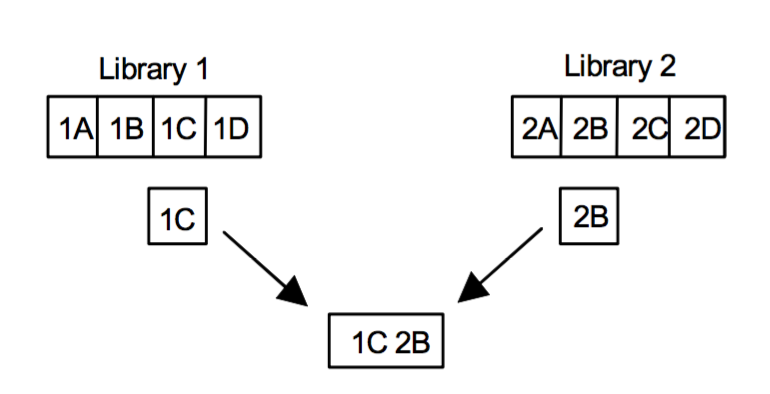
\includegraphics[width=0.7\textwidth]{fig/gene_library}
                    \caption{Schematic of antibody generation with gene libraries.}
                \end{figure}}
            

        \end{frame}
        
        \begin{frame}{Negative Selection}
            \begin{itemize}
                \only<1>{\item Based on the theory of negative selection in the Thymus;
                \item Cells that dwell in the thymus are \textit{self};
                \item T-Cells are tested against other cells;
                \item If recognition occurs, they are purged!}
                \only<2>{
                \item Cells that do not recognise self are deployed;
                \item The set of cells that exit the Thymus are called \textbf{detectors};
                \item Used for anomaly detection;
                \item Ideal for Intrusion Detection Systems.}
            \end{itemize}
        \end{frame}
        
        \begin{frame}{Negative Selection}
            Divided in two phases:
            
            \begin{itemize}
                \item Censoring phase
                \item Monitoring phase
            \end{itemize}
        \end{frame}
        
        \begin{frame}{Censoring Phase}
            \SetEndCharOfAlgoLine{}
            \scalebox{0.775}{
            \begin{algorithm}[H]
                \KwIn{$S$, a set of strings that represent \textit{self} patterns.}
                \KwIn{$\varepsilon$, the affinity threshold}
                \KwIn{$N$, number of detectors to generate}
                \KwIn{$L$, the length of an antibody string}
                
                Initialise a set of detectors $R$
                
                \While{$|R| < N$}{
                    Generate an antibody $r_{0}$
                    
                    \For{\textbf{every} $s \in S$} {
                        Calculate the similarity between $r_{0}$ and $s$\\
                        \If{similarity $\geq \varepsilon$} {
                            Discard the antibody and start over
                        }
                    }
                    
                    \If{no recognition occurred} {
                        Add the antibody to the set of detectors $R$
                    }
                }
                \textbf{return} $R$
                \caption{Pseudo-algorithm for the censoring phase.}
                \end{algorithm}}
                \centering
        \end{frame}
        
        \begin{frame}{Monitoring Phase}
            \SetEndCharOfAlgoLine{}
            \scalebox{0.775}{
            \begin{algorithm}[H]
                \KwIn{$S'$, a set of strings that represent \textit{self} patterns.}
                \KwIn{$\varepsilon$, the affinity threshold}
                \KwIn{$R$, number of detectors to generate}
                
                \ForAll{$s \in S'$} {
                    \ForAll{$r \in R$} {
                        Compute the similarity between $r$ and $s$\\
                        \If{similarty $\geq \varepsilon$} {
                            \textbf{return true}
                        }
                    }
                }
                
                \textbf{return false}

                \caption{Pseudo-algorithm for the censoring phase.}
                \end{algorithm}}
                \centering
        \end{frame}

        
        \begin{frame}{Clonal Selection}
            \begin{itemize}
                \item Immune Systems sleep when not responding to invasions;
                \item On invasion, only the most responsive antibodies wake up;
                \item Antibodies are \textbf{selected} for binding with antigens;
                \item Selected antibodies reproduce by mitosis;
                \item Mutation occurs during reproduction.
                \item Affinity Maturation
            \end{itemize}
        \end{frame}
        
        \begin{frame}{Clonal Selection}
            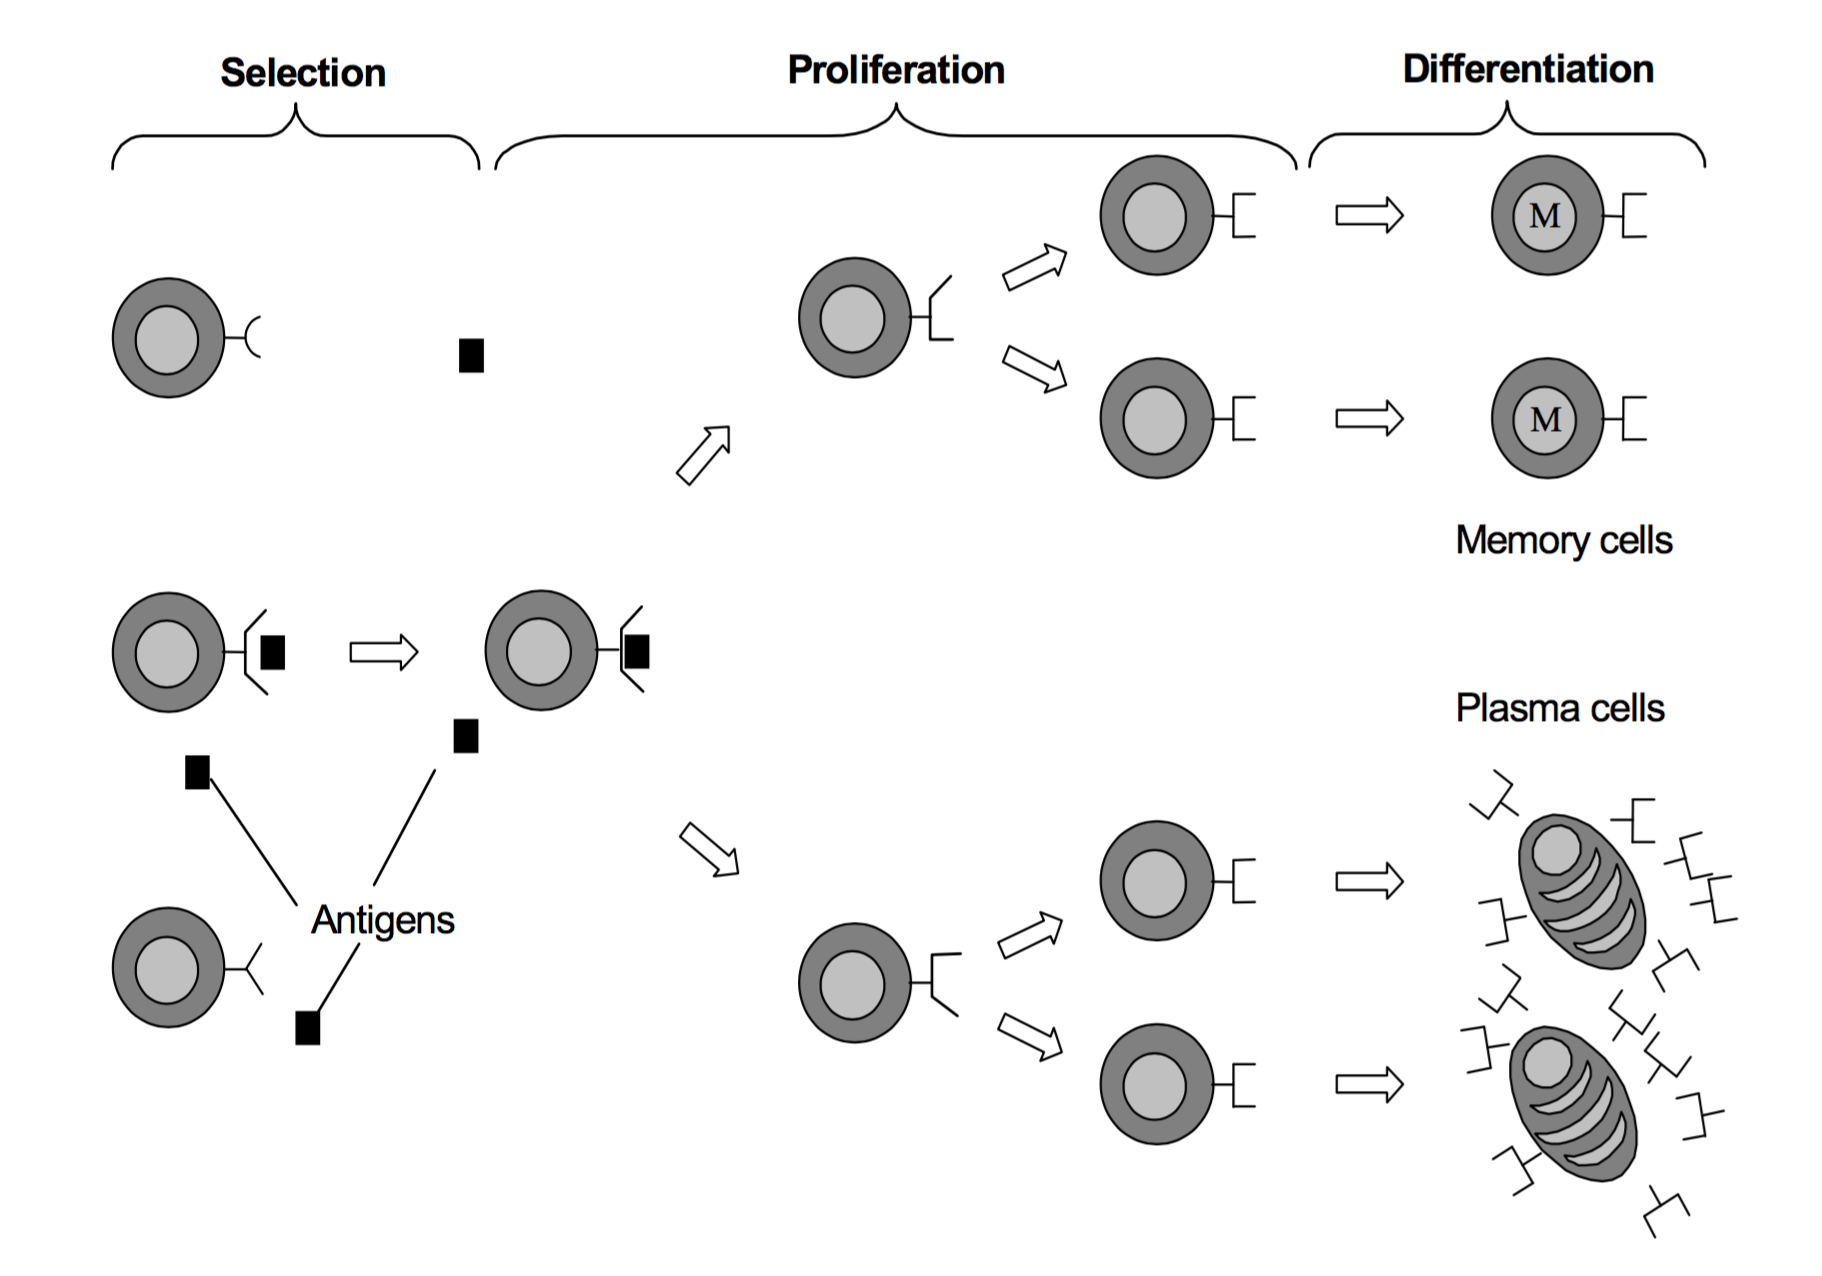
\includegraphics[width=\textwidth]{fig/clonal_selection}
        \end{frame}
        
        \begin{frame}{Clonal Selection}
            \begin{itemize}
                \item Can be done with an evolutionary approach;
                \item Fast responses when threats are known;
                \item Cells are mutated to respond to unknown threats;
                \item Process is local: occurs near infection areas.
            \end{itemize}
        \end{frame}
        
        \begin{frame}{Clonal Selection}
            \begin{itemize}
                \item Forrest's Algorithm (genetic approach)
                \item CLONALG
            \end{itemize}
        \end{frame}
        
        \begin{frame}{CLONALG}
            \SetEndCharOfAlgoLine{}
            \scalebox{0.75}{
            \begin{algorithm}[H]
                \KwIn{$S$, a set of patterns to be recognised}
                \KwIn{$e$, the number of individuals to select}
                \KwIn{$r$, the number of individuals to be replaced}
                generate initial population $P$\\

                \While{stopping condition not \textbf{true}} {
                    \For{$i \gets 0$ \textbf{to} $|S|$} {
                        Calculate the affinities between $S_{i}$ and each member of $P$\\
                        Select $e$ individuals with the highest affinities\\
                        Clone selected individuals with a rate proportional to their affinity\\
                        Mutate cloned individuals with a rate inversely proportional to their affinity\\
                        Recalculate affinities between $S_{i}$ and each member of the new population\\
                        Assign the highest affinity antibody to $M_{i}$\\
                        Replace $r$ individuals with the lowest affinities in $P$ with new ones\\ 
                    }
                }
                \textbf{return} $M$
                \caption{CLONALG, an algorithm for clonal selection.}
                \end{algorithm}}
                \centering
        \end{frame}

    \begin{frame}{Immune Networks}
        \begin{itemize}
            \item Interconnectivity between immune cells;
            \item Cells stimulate and suppress one another, they no longer need external stimulation;
            \item Network is dynamic, antibodies may die and be replaced by new ones;
            \item Antigens introduce an imbalance to the network.
        \end{itemize}
    \end{frame}
    
    \begin{frame}{Immune Networks}
        \begin{itemize}
            \item Antibodies: epitopes and paratopes;
            \item Antigens: epitopes only;
            \item Stimulation: when a paratope recognises an epitope;
            \item Supression: when an epitope is recognised by a paratope;
        \end{itemize}
    \end{frame}
    
    \begin{frame}{Immune Networks}
        \begin{itemize}
            \item Stimulation leads to reproduction;
            \item Suppression leads to death;
            \item Antibodies have a natural death rate.
        \end{itemize}
    \end{frame}    
    
    \begin{frame}{Continuous Immune Network}
        \begin{itemize}
            \item No pseudo-algorithm;
            \item It is governed by ODEs:
        \end{itemize}
        
        The concentration of each antibody $c_{i}$ can be obtained by:
        
        $$ \frac{dc_{i}}{dt} = k_{1} \left[ \sum^{N_{1}}_{j=1}{m_{ji}c_{i}c_{j}} - k_{2} \sum^{N_{1}}_{j=1}{m_{ij}c_{i}c_{j}} + \sum^{N_{2}}_{j=1}{m_{ji}c_{i}y_{j}} \right] - k_{3}c_{i} $$
        
        \center Network St $-$ Network Supp $+$ Ab St $-$ Ab death rate
        
    \end{frame}
    
    \begin{frame}{Continuous Immune Network}
        The concentration of each antibody $c_{i}$ can be obtained by:
        
        $$ \frac{dc_{i}}{dt} = k_{1} \left[ \sum^{N_{1}}_{j=1}{m_{ji}c_{i}c_{j}} - k_{2} \sum^{N_{1}}_{j=1}{m_{ij}c_{i}c_{j}} + \sum^{N_{2}}_{j=1}{m_{ji}c_{i}y_{j}} \right] - k_{3}c_{i} $$
        
        where:
        
        \begin{itemize}
            \item $m_{ij}$ is a function that expresses the stimulation of element $j$ by element $i$;
            \item $k_{1}$ is the coefficient of antibody growth;
            \item $k_{2}$ is a ratio between stimulation and suppression;
            \item $k_{3}$ is the natural death rate.
        \end{itemize}
    \end{frame}
    
    \begin{frame}{Continuous Immune Network}
        \textbf{What about the population?}
        \pause
        
        \vspace{1em}
        \begin{itemize}
            \item Assume a set of antibodies $P$
            \item We define a variable $N$ to constrain the number of elements in the network;
            \item Create a network containing $N$ random elements from $P$
            \item Compute the ODEs for each antibody in the network
            \item As antibodies die, replace them with random elements of $P$
            \item Rinse and repeat until convergence
        \end{itemize}
    \end{frame}
    
    \begin{frame}{Applications}
        
    \end{frame}
    
    \begin{frame}{Extra: Danger Theory}
		\begin{itemize}
		    \item Molecules don't distinguish \textit{self} from \textit{non-self};
            \item Stressed or damaged cells and tissues emit danger signals;
	        \item Antibodies pick up on those signals and initiate immune responses;
	        \item Danger Theory explains some facts about immunology, like tumours, auto-immune responses and beneficial bacteria found within our bodies.
	    \end{itemize}
	\end{frame}
	
    \begin{frame}
    	TODO: Set-up References
    \end{frame}     
            
    \introframe{Challenge:\\ \hfill \Large{A Movie Recommender System}}{ 
        
\includegraphics[width=85px]{fig/2001-poster}
        \hfill
        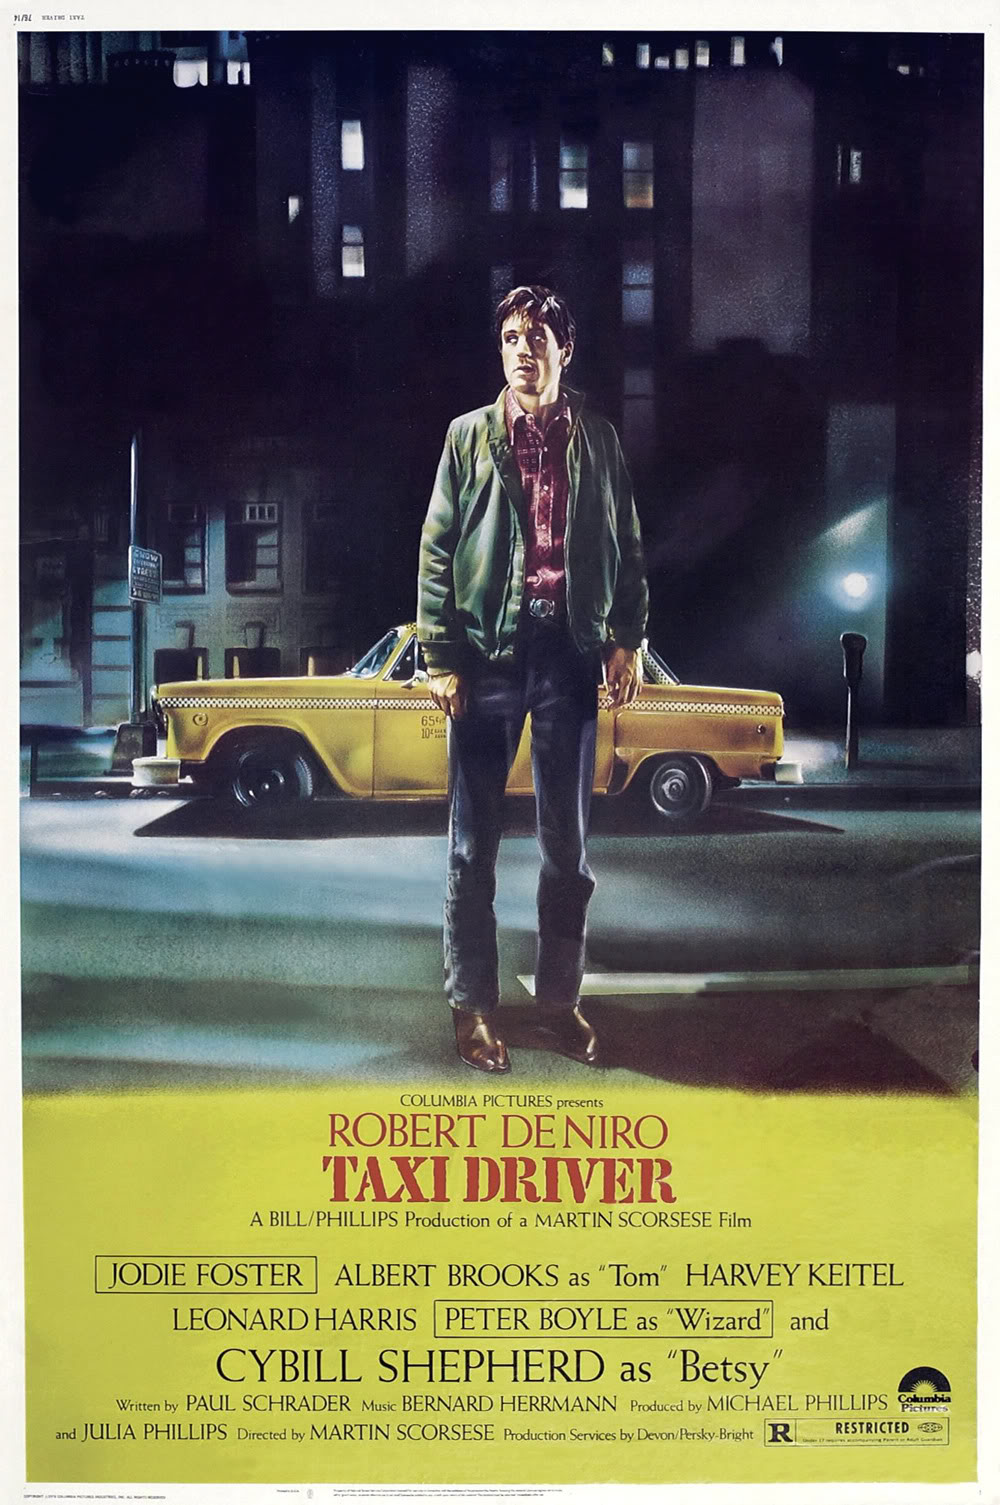
\includegraphics[width=85px]{fig/taxidriverposter}
        \hfill
        
\includegraphics[width=85px]{fig/blade_runner}}
        
\end{document}